
\documentclass[12pt]{article}

%%%%%%%%%%%%%%%%%%%%%%%%%%%%%%%%%%%%%%%%%%%%%%%%%%%%%%%%%%%%%%%%%%%%%%%%%%%%%%%%%%%%%%%%%%%%%%%%%%%%

\usepackage{amsmath,amssymb,amsthm}
\usepackage{multicol}
\usepackage{color}
\usepackage{hyperref}
\usepackage{graphicx}
\usepackage[utf8]{inputenc}
\usepackage[english]{babel}

\newcommand{\gf}{\mathfrak{g}}
\newcommand{\af}{\mathfrak{a}}

\newtheorem{Def}{Definition}[section]
\newtheorem{Cnj}[Def]{Conjecture}
\newtheorem{Prop}[Def]{Property}
\newtheorem{example}{Example}
\begin{document}

\title{Fan, splint and branching rules.}



\author{V.D.~Lyakhovsky$^1$, A.A.~Nazarov$^{1,2}$ \\
  {\small $^1$ Department of High-energy and elementary particle physics, SPb State University}\\
  {\small 198904, Saint-Petersburg, Russia}\\
  {\small e-mail: lyakh1507@nm.ru}\\
  {\small$^{2}$ Chebyshev Laboratory,}\\
  {\small Department of Mathematics and Mechanics, SPb State University}\\
  {\small 199178, Saint-Petersburg, Russia}\\
  {\small email: antonnaz@gmail.com}}
\maketitle

\begin{abstract}
Splint of root system of simple Lie algebra appears naturally in the study of (regular) embedding of reductive subalgebra. It can be used to derive branching rules. We show that the use of splint drastically simplifies the derivation of branching functions. 
\end{abstract}


\section{Introduction}
\label{sec:Introduction} 
Splint $\phi$ of root system $\Delta_1$ to root system $\Delta$ is a bijective map of roots of $\Delta_{1}$ to (proper) subset of $\Delta$ which commutes with the addition in $\Delta_{1}$ and $\Delta$. 
\begin{equation*}
\phi:\Delta_1 \longrightarrow \Delta
\end{equation*}
\begin{equation*}
\phi \circ \alpha + \beta =\phi \circ \alpha + \phi \circ \beta,
\,\,\, \alpha,\beta \in \Delta_1
\end{equation*}

Note that image $Im(\phi)$ is not required to have the properties of root system except the addition rules equivalent to the addition rules in $\Delta_{1}$ (for pre-images). The term {\it splint} was introduce in paper \cite{richter2008splints} where the classification of splints for simple Lie algebras was obtained. The conjecture of the connection splint with injection fan was stated in the same paper. 
The fan $\Gamma \subset \Delta$ as the subset of root system describing recurrent properties of branching coefficients for maximal embeddings  was introduced in \cite{lyakhovsky1996rra}. Injection fan is an efficient tool for the study of branching rules. This construction was generalized to non-maximal embeddings and infinite-dimensional Lie algebras in  \cite{2010arXiv1007.0318L, ilyin812pbc}.

In present paper we study the connection of splint with the injection fan of regular embedding of reductive subalgebra ${\mathfrak a}$. We show that (under certain conditions described in section \ref{sec:stems and multiplicity functions}) splint is a natural tool for the reduction of simple Lie algebra $\gf$-modules to the modules of subalgebra $\af\rightarrow\gf$. The use of this tool allows us to state the main result of the present paper -- the one-to-one relationship between weight multiplicities of irreducible modules of splint and branching coefficients for the reduction $L^{\mu}_{{\mathfrak g}\downarrow {\mathfrak a}}$.

\section{Injections and splints}
\label{sec:Injections and splints}

Consider a simple Lie algebra $\mathfrak{g}$ and its regular
subalgebra $\mathfrak{a}\longrightarrow \mathfrak{g%
}$ such that $\mathfrak{a}$ is a reductive subalgebra $\mathfrak{a
\subset g}$ with correlated root spaces:
$\mathfrak{h}_{\mathfrak{a}}^{\ast }\subset
\mathfrak{h}_{\mathfrak{g }}^{\ast }$. Let $\mathfrak{a}^S$ be a
semisimple summand of $\mathfrak{a}$, this means that
$\mathfrak{a}=\mathfrak{a}^S \oplus \mathfrak{a}(1)\oplus
\mathfrak{a}(1)\oplus \dots$. We shall consider $\mathfrak{a}^S$
to be a proper regular subalgebra and $\mathfrak{a}$ to be the
maximal subalgebra with $\mathfrak{a}^S$ fixed that is the rank
$r$ of $\frak{a}$ is equal to that of $\mathfrak{g}$.


$r$ , $\left( r_{\mathfrak{a}^S}\right) $ --- the rank of
$\frak{g}$ $\left( \mathrm{{resp. }\mathfrak{a}^S}\right) $ ;

$\Delta $ $\left( \Delta _{\frak{a}}\right) $--- the root system;
$\Delta ^{+} $ $\left( \mathrm{{resp. }\Delta
_{\frak{a}}^{+}}\right) $--- the positive root system (of
$\frak{g}$ and $\frak{a}$ respectively);

$S\quad \left( S_{\frak{a}}\right) $ --- the system of simple roots (of $%
\frak{g}$ and $\frak{a}$ respectively);

$\alpha _{i}$ , $\left( \alpha _{\left( \frak{a}\right) j}\right) $ --- the $%
i$-th (resp. $j$-th) simple root for $\frak{g}$ $\left( \mathrm{{resp.}\frak{a%
}}\right) $; $i=0,\ldots ,r$,\ \ $\left( j=0,\ldots
,r_{\mathfrak{a}^S}\right) $;

$W$ , $\left( W_{\frak{a}}\right) $--- the corresponding Weyl
group;

$C$ , $\left( C_{\frak{a}}\right) $--- the fundamental Weyl
chamber;

$\bar{C}, \left(\bar{C_{\frak{a}}}\right)$ --- the closure of the
fundamental Weyl chamber;

$\epsilon \left( w\right) :=\left( -1\right)
^{\mathrm{length}(w)}$;

$\rho $\ , $\left( \rho _{\frak{a}}\right) $\ --- the Weyl vector;

$L^{\mu }$\ $\left( L_{\frak{a}}^{\nu }\right) $\ --- the
integrable module of $\frak{g}$ with the highest weight $\mu $\ ;
(resp. integrable $\frak{a}$ -module with the highest weight $\nu
$ );

$\mathcal{N}^{\mu }$ , $\left( \mathcal{N}_{\frak{a}}^{\nu
}\right) $ --- the weight diagram of $L^{\mu }$ (resp.
${}L_{\frak{a}}^{\nu }$ );

$P$ (resp. $P_{\frak{a}} $) \ --- the weight lattice;

$P^{+}$ (resp. $P_{\frak{a}}^{+} $) \ --- the dominant weight
lattice;

$\cal{E}$ (resp. $\cal{E}_{\frak{a}} $) \ --- the formal algebra;

$m_{\xi }^{\left( \mu \right) }$ , $\left( m_{\xi }^{\left( \nu
\right)
}\right) $ --- the multiplicity of the weight $\xi \in P$ \ $\left( \mathrm{{%
resp. }\in P_{\frak{a}}}\right) $ in the module $L^{\mu }$ ,
(resp. $\xi \in L_{\frak{a}}^{\nu } $);

$ch\left( L^{\mu }\right) $ (resp. $\mathrm{ch}\left(
L_{\frak{a}}^{\nu }\right) $)--- the formal character of $L^{\mu
}$ (resp. $L_{\frak{a}}^{\nu } $);

$ch\left( L^{\mu }\right)
 =\frac{\sum_{w\in W}\epsilon
(w)e^{w\circ (\mu +\rho )-\rho }}
{\prod_{\alpha \in \Delta
^{+}}
\left( 1-e^{-\alpha }\right) }
$ --- the Weyl formula;

$R:=\prod_{\alpha \in \Delta ^{+}}\left( 1-e^{-\alpha }\right)
\quad
$
(resp.
$
R_{\frak{a}}:
=\prod_{\alpha \in \Delta_{\frak{a}}^{+}}
\left( 1-e^{-\alpha }\right)
$
) --- the Weyl
denominator.



Let $L^{\mu }$ be completely reducible with respect to $\frak{a}$,
\begin{equation*}
L_{\frak{g}\downarrow \frak{a}}^{\mu }=\bigoplus\limits_{\nu \in P_{\frak{a}%
}^{+}}b_{\nu }^{\left( \mu \right) }L_{\frak{a}}^{\nu }.
\end{equation*}
\begin{equation}
\pi _{\frak{a}}ch\left( L^{\mu }\right) =\sum_{\nu \in P_{\frak{a}%
}^{+}}b_{\nu }^{(\mu )}ch\left( L_{\frak{a}}^{\nu }\right) .
\label{branching1}
\end{equation}
For the modules we are interested in the Weyl formula for $\mathrm{ch}%
\left( L^{\mu }\right) $ can be written in terms of singular
elements \cite {humphreys1997introduction}
\begin{equation*}
\Psi ^{\left( \mu \right) }:=\sum\limits_{w\in W}\epsilon
(w)e^{w(\mu +\rho )-\rho },
\end{equation*}
namely,
\begin{equation}
\mathrm{ch}\left( L^{\mu }\right) =\frac{\Psi ^{\left( \mu \right)
}}{\Psi ^{\left( 0\right) }}=\frac{\Psi ^{\left( \mu \right)
}}{R}. \label{Weyl-Kac2}
\end{equation}
The same is true for submodules $\mathrm{ch}\left(
L_{\frak{a}}^{\nu }\right) $ in (\ref{branching1})
\begin{equation*}
\mathrm{ch}\left( L_{\frak{a}}^{\nu }\right) =\frac{\Psi
_{\frak{a}}^{\left(
\nu \right) }}{\Psi _{\frak{a}}^{\left( 0\right) }}=\frac{\Psi _{\frak{a}%
}^{\left( \nu \right) }}{R_{\frak{a}}},
\end{equation*}
with
\begin{equation*}
\Psi _{\frak{a}}^{\left( \nu \right) }:=\sum\limits_{w\in W_{\frak{a}%
}}\epsilon (w)e^{w(\nu +\rho _{_{\frak{a}}})-\rho _{_{\frak{a}}}}.
\end{equation*}

Applying formula (\ref{Weyl-Kac2}) to the branching rule
(\ref{branching1}) we get the relation connecting the singular
elements $\Psi ^{\left( \mu \right) }$ and $\Psi
_{\frak{a}}^{\left( \nu \right) }$ :
\begin{eqnarray}
 \frac{\sum_{w \in W}\epsilon (w )e^{w (\mu
+\rho )-\rho }}{\prod_{\alpha \in \Delta ^{+}}(1-e^{-\alpha })}
&=&\sum_{\nu \in P_{\frak{a}}^{+}}b_{\nu }^{(\mu )}\frac{%
\sum_{w \in W_{\frak{a}}}\epsilon (w )e^{w (\nu +\rho _{\frak{a}})-\rho _{%
\frak{a}}}}{\prod_{\beta \in \Delta _{\frak{a}}^{+}}(1-e^{-\beta })},
\notag  \label{eq:4} \\
\frac{\Psi ^{\left( \mu \right) }}{R}
&=&\sum_{\nu \in P_{\frak{a}}^{+}}b_{\nu }^{(\mu )}\frac{\Psi _{\frak{a}%
}^{\left( \nu \right) }}{R_{\frak{a}}}.
\label{singular main}
\end{eqnarray}

In \cite
{2010arXiv1007.0318L} it was proven that branching coefficients $b_{\xi
}^{\left( \mu \right) }$ corresponding to the injection $\frak{a}%
\hookrightarrow \frak{g}$ are subject to the set of recurrent relations:
\begin{equation}
\begin{array}{c}
b_{\xi }^{\left( \mu \right) }=-\frac{1}{s\left( \gamma _{0}\right) }\left(
\sum_{u\in U}\epsilon (u)\;\dim \left( L_{\frak{a}_{\perp }}^{\mu _{\frak{a}%
_{\perp }}\left( u\right) }\right) \delta _{\xi -\gamma _{0},\pi _{%
\widetilde{\frak{a}}}(u(\mu +\rho )-\rho )}+\right.  \\
\left. +\sum_{\gamma \in \Gamma _{\widetilde{\frak{a}}\rightarrow \frak{g}%
}}s\left( \gamma +\gamma _{0}\right) b_{\xi +\gamma }^{\left( \mu \right)
}\right) .
\end{array}
\label{recurrent rel}
\end{equation}
where $\frak{a}_{\perp }$ is the subalgebra determined by the roots of $\frak{g}$ orthogonal to roots of $\frak{a}$
\begin{eqnarray}
\Delta _{\frak{a}_{\perp }} &:&=\left\{ \beta \in \Delta _{\frak{g}}|\forall
h\in \frak{h}_{\frak{a}};\beta \left( h\right) =0\right\} ,
\label{delta a ort}
\end{eqnarray}
\begin{eqnarray}
\widetilde{\frak{a}_{\perp }} :=\frak{a}_{\perp }\oplus \frak{h}_{\perp }
\qquad
\widetilde{\frak{a}} :=\frak{a}\oplus \frak{h}_{\perp }
\end{eqnarray}
and $\pi$ is the projection operator. When the injection is maximal the projection becomes trivial and the relation (\ref{recurrent rel}) is simplified:
\begin{equation}
\begin{array}{c}
b_{\xi }^{\left( \mu \right) }=-\frac{1}{s\left( \gamma _{0}\right) }\left(
\sum_{u\in W}\epsilon (u) \delta _{\xi -\gamma _{0}, u(\mu +\rho )-\rho }+\right.  \\
\left. +\sum_{\gamma \in \Gamma _{\frak{a}\rightarrow \frak{g}%
}}s\left( \gamma +\gamma _{0}\right) b_{\xi +\gamma }^{\left( \mu \right)
}\right) .
\end{array}
\label{recurrent relation max}
\end{equation}
The recursion is goverened by the set $\Gamma _{\frak{a}%
\rightarrow \frak{g}}$ called the injection fan. The latter is defined by the
carrier set $\left\{ \xi \right\} _{\frak{a}\rightarrow \frak{g}}$ for the
coefficient function $s(\xi )$
\begin{equation*}
\left\{ \xi \right\} _{\frak{a}\rightarrow \frak{g}}:=\left\{
\xi \in P_{\frak{a}}|s(\xi )\neq 0\right\}
\end{equation*}
appearing in the expansion
\begin{equation}
\prod_{\alpha \in \Delta ^{+}\setminus \Delta _{\frak{a}}^{+}}\left( 1-e^{
-\alpha }\right) =-\sum_{\gamma \in P_{%
\frak{a}}}s(\gamma )e^{-\gamma };\quad
\label{product}
\end{equation}

Now we remind two definitions introduced in \cite{richter2008splints}
\begin{Def}
Suppose $\Delta_0$ and $\Delta$ are root systems with the corresponding weight lattices $P_0$ and $P$.  Then $\phi$ is an ``embedding'', 
\begin{equation}
\phi:\left\{
\begin{array}{l}
\Delta_0\hookrightarrow\Delta,\\
P_0 \hookrightarrow P,
 \end{array}
\right.
\end{equation}
if \\
\noindent
(a) it injects $\Delta_0$ in $\Delta$, and \\
\noindent
(b) acts homomorphically with respect to the vector groups in $P_0$ and $P$:
$$\phi(\gamma)=\phi(\alpha)+\phi(\beta)$$
for any triple $\alpha,\beta,\gamma\in P_0$ such that $\gamma=\alpha+\beta$.
\end{Def}
$\phi$ induces an injection of formal algebras $ :{\cal{E}}_0 \longrightarrow \cal{E}$ and for the image ${\cal{E}}_i=Im_{\phi}\left( {\cal{E}}_0\right)$ one can consider its inverse
$\phi^{-1}:{\cal{E}}_i \longrightarrow {\cal{E}}_0$. 

 Notice that one must distinguish two classes of embeddings: when the scalar product (defined by the Killing form) in the root space $P_0$ is invariant with respect to $\phi$ and when it is not $\phi$-invariant. The first embedding is called "metric" 
, the second -- "nonmetric". 
\begin{Def}
A root system $\Delta$ "splinters'' as $(\Delta_1,\Delta_2)$ if there are two embeddings
$\phi_1:\Delta_1\hookrightarrow\Delta$ and $\phi_2:\Delta_2\hookrightarrow\Delta$
where (a) $\Delta$ is the disjoint union of the images of $\phi_1$ and $\phi_2$ and
(b) neither the rank of $\Delta_1$ nor the rank of $\Delta_2$ exceeds the rank of $\Delta$.
\end{Def}
It is equivalent to say that $(\Delta_1,\Delta_2)$ is a "splint'' of $\Delta$ and we shall denote this by $\Delta \approx (\Delta_1,\Delta_2)$.
Each component $\Delta_1$ and $\Delta_2$ is a "stem'' of the splint $(\Delta_1,\Delta_2)$.

In \cite{richter2008splints} it was indicated that the injection fan technique used in \cite{lyakhovsky1996rra} is close to that of splints.

To demonstrate the relations between these instruments consider the case where
one of the stems $\Delta_1=\Delta_{\frak{a}}$ is a root system of a regular reductive subalgebra  $\frak{a}\hookrightarrow\frak{g}$. Then the second stem is $\Delta_{\frak{s}}:=\Delta_2=\Delta \setminus \Delta _{\frak{a}}$ can be translated into the product (\ref{product}) and defines the injection fan $\Gamma_{\frak{a}\hookrightarrow\frak{g}}$.

Thus we see that
\begin{Cnj}
Each splint of the type $\Delta \approx (\Delta_{\frak{a}},\Delta_{\frak{s}})$ defines an injection fan with the carrier $\left\{ \xi \right\} _{\frak{a}\rightarrow \frak{g}}$ fixed by the product
\begin{equation}
\prod_{\beta \in  \Delta _{\frak{s}}^{+}}\left( 1-e^{
-\beta }\right) =-\sum_{\gamma \in P} s(\gamma )e^{-\gamma }\quad
\label{splint product}
\end{equation}
\end{Cnj}
In this case we say that the subalgebra $\frak{a}\hookrightarrow\frak{g}$ splinters $\Delta$ (and call $\frak{a}$ the "splinting subalgebra" of $\frak{g}$). In
\cite{richter2008splints} the splints are classified (see Appendix) and in the first three types one can easily see that one of the stems corresponds to a splinting subalgebra.

\section{How stems define multiplicity functions}
\label{sec:stems and multiplicity functions}

In this Section we consider the situation where  the splinting subalgebra is "larger"
than the Lie algebra $\frak{s}$ defined by the root system $\Delta_{\frak{s}\,0}=CoIm_{\phi} \left( \Delta_{\frak{s}}\right)$
(the details will be given below). In such a case to find branching coefficients for a splinting 
injection $\frak{a}\hookrightarrow\frak{g}$ means to find weight multiplicities for an irreducible $\frak{s}$-module $L^{\nu}_{\frak{s}}$ with 
the fixed highest weight $\nu$. Notice that $\frak{s}$ must not be a subalgebra of $\frak{g}$.

Let us return to relation (\ref{singular main}) and multiply both sides by $R_{\frak{a}}$: 
\begin{eqnarray}
 \frac{1}{\prod_{\beta \in \Delta_{\frak{s}} ^{+}}(1-e^{-\beta })}\Psi_{\frak{g}} ^{\left( \mu \right) }
&=&
\sum_{\nu \in P_{\frak{a}}^{+}}b_{\nu }^{(\mu )}\Psi _{\frak{a}%
}^{\left( \nu \right) }.
\label{singular main-2}
\end{eqnarray}
Here the first factor in the l.h.s. is the inverse of the fan $\Gamma _{\frak{a}%
\rightarrow \frak{g}}$. 
Consider the highest weight module $L^{\nu}_{\frak{s}}$. An embedding
$\phi:\Delta_{\frak{s}\,0} \longrightarrow \Delta_{\frak{g}} $  sends the singular element         $\Psi_{\frak{s}} ^{\left( \nu \right)}$ into $ \Psi_{\frak{g}} ^{\left( \mu \right) }$.
Applying the inverse morphism $\phi^{-1}$ to the product 
$\left(\prod_{\beta \in \Delta_{\frak{s}} ^{+}}(1-e^{-\beta })\right)^{-1}\phi\left(\Psi_{\frak{s}} ^{\left( \nu \right)}\right)$  
 one obtains the character of the module $L^{\nu}_{\frak{s}}$,

\begin{equation}
 \phi^{-1}\left( \frac{1}{\prod_{\beta \in \Delta_{\frak{s}} ^{+}}(1-e^{-\beta })}\phi\left(\Psi_{\frak{s}} ^{\left( \nu \right)}\right)\right)
 =
 \frac{1}{\prod_{\beta \in \Delta_{\frak{s}\left(0\right)} ^{+}}(1-e^{-\beta })}\Psi_{\frak{s}} ^{\left( \nu \right)}
 =
 \mathrm{ch}\left( L_{\frak{s}}^{\nu }\right).
\label{inverse for stem}
\end{equation}
Our task is to prove that the singular element $\Psi_{\frak{g}} ^{\left( \mu \right) }$ contains the element $\Psi_{\frak{g}} ^{\left( \xi \right) }$ for a module $L^{\xi}_{\frak{s}}$ uniquely defined by $L^{\mu}_{\frak{g}}$ and that the branching coefficients $b_{\nu }^{(\mu )}$ in the r.h.s. of (\ref{singular main-2})  coincide with multiplicities $m_{\zeta}^{\left( \xi \right) }$ of the weights of $L^{\xi}_{\frak{s}}$. 

For a highest weight irreducible module $L^{\mu}_{\frak{g}}$ the singular element $\Psi_{\frak{g}} ^{\left( \mu \right) }$ is an element of $\cal{E}$ corresponding to the shifted Weyl-orbit of the weight $\left( \mu + \rho \right) \in P^+$ and the sign function $\epsilon\left( w \right)$. It is convenient to use also unshifted singular elements  
\begin{equation}
 \Phi^{\left( \mu \right)}:= \Psi^{\left( \mu \right) }e^{\rho}.
 \label{definition Phi}
\end{equation}
In these terms the relation (\ref{singular main-2}) looks like
\begin{equation}
 \frac{e^{\rho_{\frak{g}}-\rho_{\frak{a}}}}{\prod_{\beta \in \Delta_{\frak{s}} ^{+}}(1-e^{-\beta })}\Phi_{\frak{g}} ^{\left( \mu \right) }
=
\sum_{\nu \in P_{\frak{a}}^{+}}b_{\nu }^{(\mu )}\Phi _{\frak{a}%
}^{\left( \nu \right) }.
\label{singular main-3}
\end{equation}
The orbit that corresponds to $\Phi_{\frak{g}} ^{\left( \mu \right) }$ is completely defined by 
the set of edges $\left\{ \lambda_{i}\right\}_{i=1,\dots,r}$ adjusted to the end of the highest weight vector $\mu + \rho$. Let $\mu=\sum m_i \omega_i$ then 
\begin{equation}
 \lambda_i=-\left( m_i +1\right)\alpha_i .\quad i=1,\dots,r
\label{edge}
\end{equation}
Each weight $\mu + \rho + \lambda_i $ bears the sign coefficient $(-)$ in the singular element. The defining property of $\Phi_{\frak{g}} ^{\left( \mu \right) }$ is as follows. Consider any pair of edges $\lambda_i,\lambda_j$ and the corresponding weights $\mu + \rho $, $\mu + \rho + \lambda_i $ and $\mu + \rho + \lambda_j $. Apply the reflection $s_{\alpha_i}$ (or $s_{\alpha_j}$),  
\begin{equation}
 s_{\alpha_i}\circ
 \left\{
\begin{array}{l}
\left( \mu + \rho  \right)\\
\left( \mu + \rho + \lambda_i \right)\\
\left( \mu + \rho + \lambda_j \right)
 \end{array}
\right.
= 
  \left\{
\begin{array}{l}
\left( \mu + \rho + \lambda_i \right)\\
\left( \mu + \rho  \right)\\
\left( \mu + \rho + \lambda_i -  (m_j + 1) s_{\alpha_i}\circ \alpha_j\right)
 \end{array}
\right.
 \label{reflected triple}
\end{equation}

\begin{Prop}
 The edge $\lambda_{i,j}$ of $\Phi_{\frak{g}} ^{\left( \mu \right) }$ starting at the weight $\left( \mu + \rho + \lambda_i \right)$ along the root $- s_{\alpha_i}\circ \alpha_j$ has the same length in $( s_{\alpha_i}\circ \alpha_j )$ as $\lambda_j$ has in $\alpha_j$.
(The same is true for the edge $\lambda_{i,j}$, its length in $( s_{\alpha_j}\circ \alpha_i )$  is equal to the length of $\lambda_i$ in $\alpha_i$.)
\label{diagram property}
\end{Prop}
  In $\Phi_{\frak{g}} ^{\left( \mu \right) }$ the elements $e^{\left( \mu + \rho + \lambda_i -  (m_j + 1) s_{\alpha_i}\circ \alpha_j\right)}$ and  $e^{\left( \mu + \rho + \lambda_j -  (m_i + 1) s_{\alpha_j}\circ \alpha_i\right)}$
have the sign $(+)$.

From now on we consider splints for simple Lie algebras of the first three types according to the classification in \cite{richter2008splints}: 
$$\begin{array}{c c||c|c}
\hbox{type}
& \hspace{0.25 in}\Delta\hspace{0.25 in} & \hspace{0.25 in}\Delta_{\frak{a} }\hspace{0.25 in} & \hspace{0.25 in}\Delta _{\frak{s}}\hspace{0.25 in} \\
\hline
\hline
\hbox{(i)}     & G_2 & A_2 & A_2 \\
& F_4 & D_4 & D_4 \\
\hline
\hbox{(ii)} & B_r (r\geq 2) & D_r & rA_1 \\
    & C_r (r\geq 3) & D_r  & rA_1 \\
\hline
\hbox{(iii)}    & A_r (r\geq 2) & A_{r-1} & r A_1 \\
    & B_2 & A_1 & A_2 \\
\end{array}$$

Each row in the table gives a splint $(\Delta_{\frak{a} },\Delta_{\frak{s} })$ of the simple root system $\Delta$.
For these types:  
(i) Both $\Delta_{\frak{a} }$ and $\Delta_{\frak{s} }$ are embedded metrically, and $\Delta_{\frak{a} }\cong\Delta_{\frak{s} }$. 
(ii) Both $\Delta_{\frak{a} }$ and $\Delta_{\frak{s} }$ are embedded metrically, but $\Delta_{\frak{a} }$ and $\Delta_{\frak{s} }$ are not isomorphic.
(iii) Only $\Delta_{\frak{a} }$ is embedded metrically.

Splints induce a decomposition of the set $S=S_{\frak{c}} \cup S_{\frak{d}}$ where $S_{\frak{c}}=S \cap S_{\frak{a}}$ and $S_{\frak{d}}=S \cap S_{\frak{s}}$. It is easy to check that for all the splints we are interested in   the subset $S_{\frak{d}}$ is nonempty. It follows that in the set $\left\{ \lambda_{i}\right\}_{i=1,\dots,r}$ one can always find simple roots $\beta_k \in \Delta_{\frak{s}}$ and that the orbit corresponding to $\Phi_{\frak{g}} ^{\left( \mu \right) }$ contains edges 
\begin{equation}
 \lambda_k=-\left( m_k +1\right)\beta_k 
\label{beta edge}
\end{equation}
attached to the weight $\mu + \rho$. As far as $\Delta_{\frak{a}} $ is a root system and for any pair of simple roots from $S_{\frak{c}}$ the singular element $\Phi_{\frak{g}} ^{\left( \mu \right) }$ is a singular element for a set of $\frak{a}$-modules the property \ref{diagram property} is fulfilled. Consider $\alpha_l \in S_{\frak{c}}$ with the corresponding edge $ \lambda_l=-\left( m_l +1\right)\alpha_l $ and a root $\beta_l \in \Delta_{\frak{s}}$ whose  coimage in $\Delta_{\frak{s}0}$ is simple. The root $\beta_l $ is not simple in $\Delta$. Firstly suppose that $\beta_l =\alpha_l + \beta_k$. It is easily seen that the corresponding edge intersects the boundary plane of the fundamental chamber $\bar{C_{\frak{a}}}$ orthogonal  to the root  $\alpha_l$:
\begin{equation}
s_{\alpha_l}\left( \mu + \rho - p\beta_l\right)=s_{\alpha_l}\left( \mu + \rho \right) - p s_{\alpha_l}\beta_l=\mu + \rho - p\beta_l
\label{intersection}
\end{equation}
\begin{equation}
\mu + \rho - s_{\alpha_l}\left( \mu + \rho \right)=\left( m_l +1\right)\alpha_l =\left( m_l +1\right)\beta_l - \left( m_l +1\right)\beta_k=p\beta_l  - ps_{\alpha_l}\beta_l
\label{intersection}
\end{equation}
It follows that $p=\left( m_l +1\right)$ and $s_{\alpha_l}\beta_l=\beta_k$. Now apply the operator $s_{\beta_k}$ and find that the edge along the root $s_{\beta_k}\alpha_l$ attached at the weight $s_{\beta_k}(\mu + \rho)$ is also equal to $ -p s_{\beta_k}\alpha_l$. This means that for the triple of roots $\beta_k,\beta_l$ and $s_{\beta_k}\alpha_l$ in $\Delta_{\frak{s}}$ the edges $\lambda_k=-\left( m_k +1\right)\beta_k  $, $\lambda_l=-\left( m_l +1\right)\beta_l$ and $\lambda_{kl}=-\left( m_l +1\right)s_{\beta_k}\alpha_l$ have the property \ref{diagram property}. One can continue this procedure further in the 2-dimensional subspace    fixed by the roots $\beta_k$ and $beta_l$ and find the set of formal exponents that being supplied with the corresponding sign factors compose the coimage of the singular element of a module for the subalgebra in $\frak{s}$ (this subalgebra has rank $r=2$).    

The same can be proven for any positive root $\beta_l \in \Delta$ that is simple in $\Delta_{\frak{s}0}$ and correspondingly for any $r=2$ subalgebra in $\frak{s}$. The latter means that to "find" a singular element of $\frak{s}$-module in $\Phi_{\frak{g}} ^{\left( \mu \right) }$ it is necessary to incorporate in it additional formal elements corresponding to the weights belonging to the boundary of the chamber $\bar{C_{\frak{a}}}$. 

Now let us return to the relation (\ref{singular main-3}). One can add to $\Phi_{\frak{g}} ^{\left( \mu \right) }$ pairs of necessary formal elements with the opposite  signs.  Notice that all the additional weights belong to the boundaries of $\bar{C_{\frak{a}}}$. To form a singular element for an $\frak{s}$-module one must attribute to these weights the fixed signs. The same elements with the opposite signs are to be referred to the neighbor Weyl chambers of $\bar{C^{(l)}_{\frak{a}}}$ (the latter are connected with the main one by simple reflections $s_{\alpha_l}$). In fact one can repeat the procedure of finding additional singular weights in any Weyl chamber $\bar{C^{(m)}_{\frak{a}}}$ and in them additional singular weights always have the signs opposite to that in their neighbors. Thus without changing in fact the element $\Phi_{\frak{g}} ^{\left( \mu \right) }$ one can present it as a sum  
\begin{equation}
\Phi_{\frak{g}} ^{\left( \mu \right) }=\sum_{w \in W_{\frak{a}}} w \circ \left(e^{\rho_{\frak{a}}}\Psi^{\widetilde{\mu} + \rho_{\frak{s}}}\right)
\label{singular final}
\end{equation}
where the weight $\widetilde{\mu}=\sum m_k \omega_{\frak{s}}^k$ has the same Dynkin labels $m_k$ as in the corresponding decomposition $\mu=\sum m_k \omega_{\frak{g}}^k$. 
The decomposition (\ref{singular final}) provides the possibility to apply the factor
$\left(\prod_{\beta \in \Delta_{\frak{s}} ^{+}}(1-e^{-\beta })\right)^{-1}$ to each summand of the singular element $\Phi_{\frak{g}} ^{\left( \mu \right) }$ separately because the sets of weights from different Weyl summands do not intersect. Taking into account the isomorphism $\phi$ one can see that in the main Weyl chamber $\bar{C_{\frak{a}}}$ the set of weights generated by the factor $\left(\prod_{\beta \in \Delta_{\frak{s}} ^{+}}(1-e^{-\beta })\right)^{-1}$ is isomorphic with the weight diagram of the $\frak{s}$-module $L^{\widetilde{\mu}}_{\frak{s}}$. Finally one must restrict relation (\ref{singular main-3}) to 
$\bar{C_{\frak{a}}}$ and obtain the main result:
\begin{Prop}
\begin{equation}
 \frac{e^{\rho_{\frak{g}}}}{\prod_{\beta \in \Delta_{\frak{s}} ^{+}}(1-e^{-\beta })}\left(\Psi^{\widetilde{\mu} + \rho_{\frak{s}}}\right)
=e^{\rho_{\frak{g}}}\left( \phi^{-1}\left( \mathcal{N}_{\frak{a}}^{\widetilde{\mu}
}\right)  \right)
=
\sum b_{\nu }^{(\mu )}e^{\nu}.
\label{singular main-4}
\end{equation}
\end{Prop}

\section{Examples}
\label{sec:examples}
\begin{example}
  Consider Lie algebra $A_{2} (\bf{sl}(3))$ and branching of its irreducible module $L^{(3,2)}$ into the modules of reductive subalgebra $A_{1}\oplus u(1)$ with root system spanned by first simple root of $A_{2}$. Singular element of $L^{(3,2)}$ is decomposition into the sum of splint images of singular elements of $A_{1}\oplus A_{1}$-modules and branching coefficients coincide weight multiplicities of $A_{1}\oplus A_{1}$-module (see Fig. \ref{fig:a2_splint}).

  \begin{figure}[h!bt]
  \noindent\centering{
   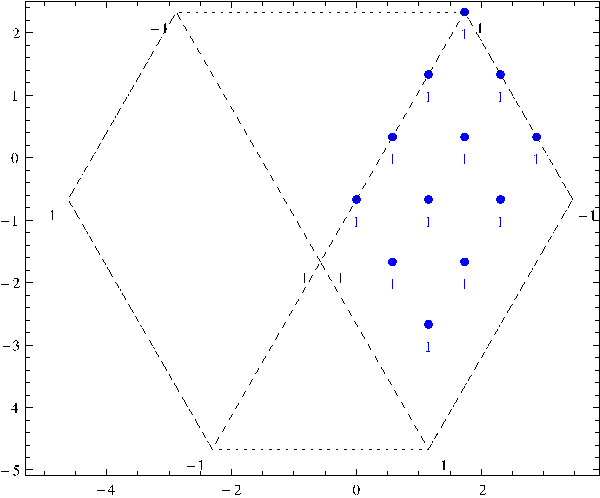
\includegraphics[width=120mm]{a2-a1}
  }
  \caption{Weyl group orbit (dotted) producing singular element of $A_{2}$-module $L^{(3,2)}$ and its decomposition into the sum of splint images of singular elements of $A_{1}\oplus A_{1}$-modules (dashed). Weight multiplicities of $A_{1}\oplus A_{1}$-module coincide with branching coefficients for the reduction $L^{(3,2)}_{A_{2}\downarrow A_{1}\oplus u(1)}$.}

 \label{fig:a2_splint}
\end{figure}
\end{example}
\begin{example}
  Now consider Lie algebra $B_{2} (\bf{so}(5))$ and branching of its irreducible module $L^{(3,2)}$ into the modules of reductive subalgebra $A_{1}\oplus u(1)$ with root system spanned by first simple root of $B_{2}$. Singular element of $L^{(3,2)}$ is decomposition into the sum of splint images of singular elements of $A_{2}$-modules and branching coefficients coincide weight multiplicities of $A_{2}$-module (see Fig. \ref{fig:b2_splint}).

  \begin{figure}[h!bt]
  \hspace*{-1.5cm}

   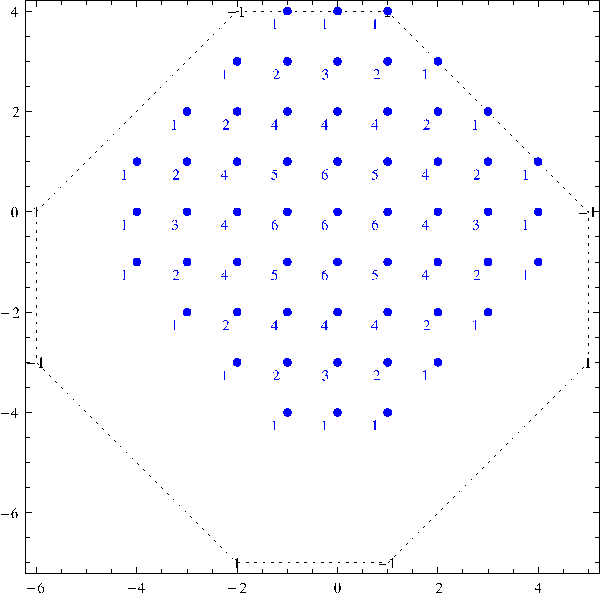
\includegraphics[width=75mm]{b2}
   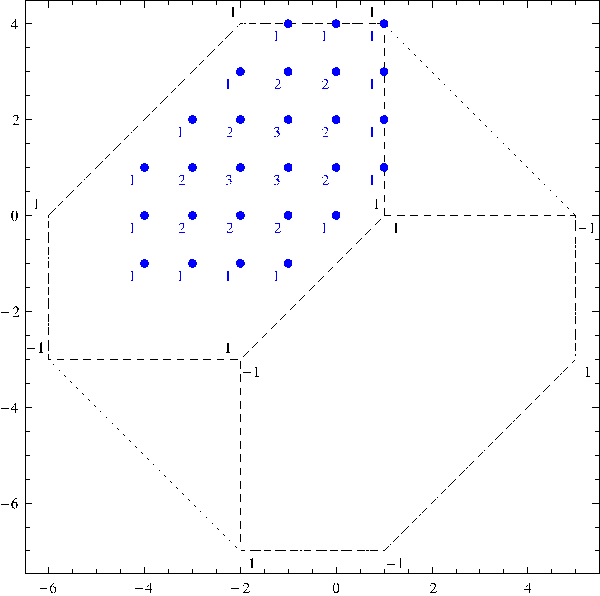
\includegraphics[width=75mm]{b2-a2-a1}
  \caption{$B_{2}$-module $L^{(3,2)}$ is shown on the left. Weight multiplicities are indicated. Contour of singular element is shown by dotted line. Right figure represents the decomposition of  $L^{(3,2)}$-singular element into the sum of splint images of singular elements of $A_{2}$-modules (dashed). Weight multiplicities of $A_{2}$-module coincide with branching coefficients for the reduction $L^{(3,2)}_{B_{2}\downarrow A_{1}\oplus u(1)}$.}

 \label{fig:b2_splint}
\end{figure}
\end{example}
\begin{example}
   Lie algebra $G_{2}$ has regular subalgebra $A_{2}$ with root system built on long roots of $G_{2}$. Consider branching of its irreducible module $L^{(3,2)}$ into the modules of reductive subalgebra $A_{2}$. Singular element of $L^{(3,2)}$ is decomposition into the sum of splint images of singular elements of $A_{2}$-modules and branching coefficients coincide weight multiplicities of $A_{2}$-module (see Fig. \ref{fig:g2_splint}).


  \begin{figure}[h!bt]
  \noindent\centering{
   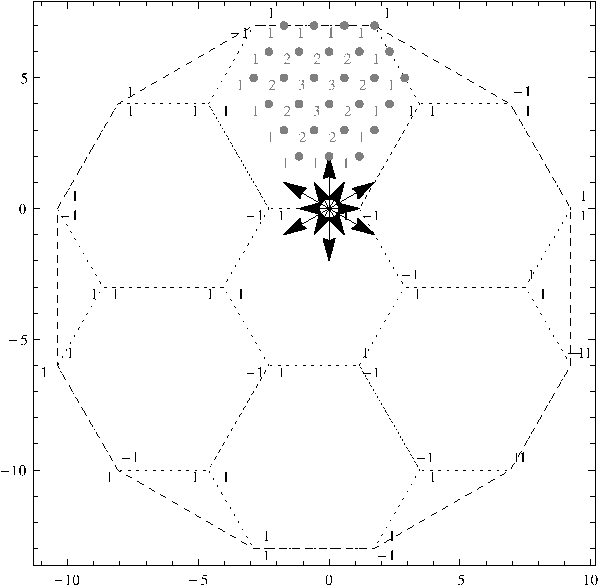
\includegraphics[width=120mm]{g2}
  }

  \caption{Weyl group orbit (dotted) producing singular element of $G_{2}$-module $L^{(3,2)}$ and its decomposition into the sum of splint images of singular elements of $A_{2}$-modules (dashed). Weight multiplicities of $A_{2}$-module coincide with branching coefficients for the reduction $L^{(3,2)}_{G_{2}\downarrow A_{2}}$.}


 \label{fig:g2_splint}
\end{figure}

\end{example}

\section{Conclusions}
\label{sec:conclusions}


\section*{Acknowledgements}
\label{sec:acknowledgements}

The work of A.A.~Nazarov is supported by the Chebyshev Laboratory
(Department of Mathematics and Mechanics, Saint-Petersburg State
University) under the grant 11.G34.31.0026 of the Government of the
Russian Federation.

\bibliography{bibliography}{}
\bibliographystyle{utphys}

%%%%%%%%%%%%%%%%%%%%%%%%%%%%%%%%%%%%%%%%%%%%%%%%%%%%%%%%%%%%%%%
%%\begin{thebibliography}{99}
%%\bibitem{2010arXiv1007.0318L}
%%V. Lyakhovsky and A. Nazarov, ТRecursive algorithm and branching
%%for nonmaximal embeddingsУ, J. Phys. A: Math. Theor. 44 (2011),
%%075205. arXiv:1007.0318 [math.RT].
%%
%%\bibitem{Richter}D. A. Richter,"Splints of classical root systems",
%%arXiv:0807.0640v1 [math.RT].
%%
%%\bibitem{LyakhMel} V. D. Lyakhovsky and S. Yu Melnikov, "Recursion relations and branching rules for simple Lie algebras", J. Phys. A: Math. Gen. 29 (1996) 1075-1087.
%%
%%\end{thebibliography}
%%%%%%%%%%%%%%%%%%%%%%%%%%%%%%%%%%%%%%%%%%%%%%%%%%%%%%%%%%%%%%%


\end{document}
